\chapter{Game Analysis}

In Chapter \ref{GameDescription}, we briefly explored the rules and gameplay mechanics of Quoridor.
As we progress, this chapter aims to deepen our understanding by analyzing Quoridor from a
theoretical and computational perspective.

In this chapter will classify Quoridor within the realm of strategic games, examine its game tree,
state-space and tree complexity, and explore the implications of these factors on gameplay and
artificial intelligence application.

\section{Classification of Quoridor}

Quoridor can be characterized as a discrete, deterministic, zero-sum, sequential, game with perfect
information (\cite{Glendenning2002MasteringQ}) , and therefore, a combinatorial game (\cite{GameTheoryBook})

\subsection{Discrete}
In every turn, each player has a finite number of moves and wall placements. These are limited by the
game state (already placed walls and moved pawns) and the rules of the game. The game-tree of Quoridor
has finite number of nodes (e.g \ref{fig:GameTree})

\subsection{Deterministic}
Quoridor has no random elements or chance involved in the gameplay. Every outcome and situation
is a direct result of the players' decisions and strategies. There's no dice rolling,
card drawing, or any other mechanism that introduces randomness.

\subsection{Zero-sum}
In Quoridor, when a player makes a move that brings them closer to winning (like advancing their pawn
or placing a wall effectively), it inherently puts the opponent at a disadvantage. Therefore, any
positive progress for a player translates into a negative impact for their opponent. This reciprocal
relationship of gain and loss between the players is what characterizes Quoridor as a \textbf{zero-sum} game.

\subsection{Perfect Information}
Every aspect of its gameplay are completely visible and known to all players at all times. This means
that the positions of the pawns and the placements of the walls on the board are always in full view,
allowing players to make strategic decisions based on the entire state of the game.

\newpage

\section{Game-Tree}


\begin{figure}[h]
    \centering
    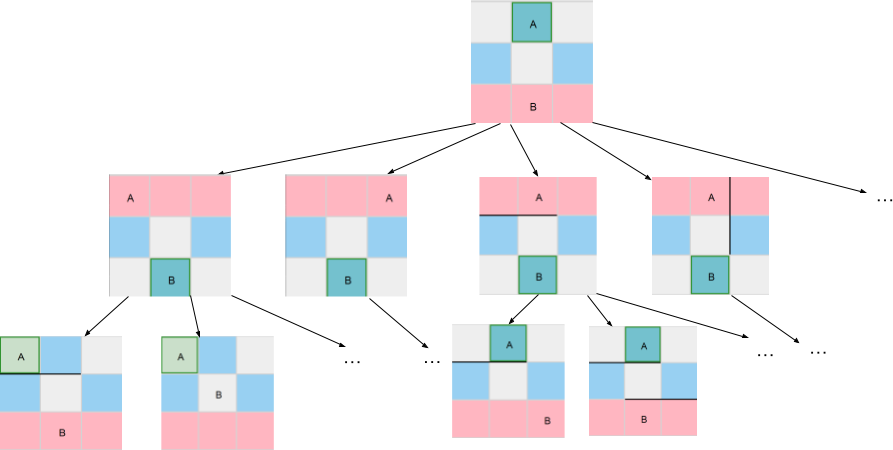
\includegraphics[scale=0.45]{../img/GameBoard/game_tree.png}
    \caption{A partial game tree for a 3x3 game board.}
    \label{fig:GameTree}
\end{figure}

\begin{figure}[h]
    \centering
    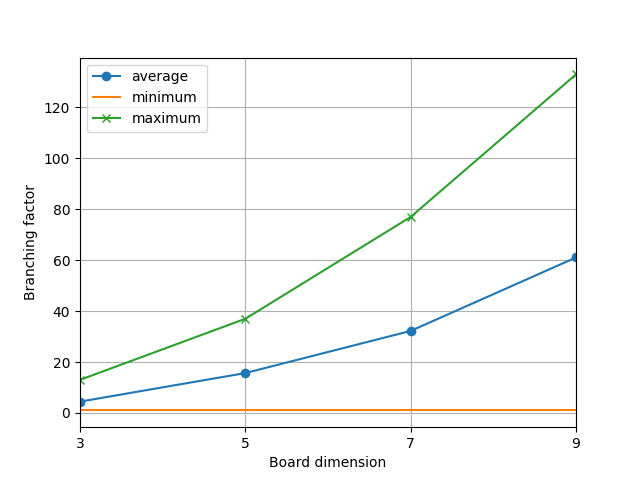
\includegraphics[scale=0.6]{../img/branching_factor.png}
    \caption{Branching factor for boards of different sizes}
    \label{fig:BranchingFactor}
\end{figure}